\documentclass[11pt,a4paper]{article}
\usepackage[utf8]{inputenc}
\usepackage[vietnamese]{babel}
\usepackage{amsmath,amssymb}
\usepackage[version=4]{mhchem}
\usepackage{geometry}
\geometry{top=1.5cm,bottom=1.2cm,left=1.4cm,right=1.4cm,headheight=28pt,headsep=12pt,footskip=18pt}
\usepackage{graphicx}
\usepackage{xcolor}
\usepackage{tabularx}
\usepackage{array}
\usepackage{colortbl}
\usepackage{tikz}
\usepackage{fancyhdr}
\usepackage{enumitem}

\definecolor{hfRed}{HTML}{D32F2F}
\definecolor{hfGreen}{HTML}{8BC390}
\definecolor{mainGreen}{HTML}{2E7D32}
\definecolor{solBlue}{HTML}{1565C0}
\definecolor{tableGreen}{HTML}{E8F5E9}

\usepackage{ex_test}

\pagestyle{fancy}
\fancyhf{}
\renewcommand{\headrulewidth}{0.75pt}
\renewcommand{\headrule}{\hbox to\headwidth{\color{hfGreen}\leaders\hrule height \headrulewidth\hfill}}
\renewcommand{\footrulewidth}{0.75pt}
\renewcommand{\footrule}{\hbox to\headwidth{\color{hfGreen}\leaders\hrule height \footrulewidth\hfill}}

\fancyhead[L]{\small\itshape\color{hfRed}Tài liệu lưu hành nội bộ}
\fancyhead[R]{\small\color{hfRed}Thầy \textbf{TRẦN VĂN THẠNH} - 0777.470.803}

\fancyfoot[L]{\footnotesize\itshape\color{hfRed}CS1: 6/15 Nguyễn Hoàng, P. Kim Long, TP Huế \quad|\quad CS2: 24 Đặng Thái Thân, TP Huế}
\fancyfoot[R]{\small\textbf{\color{hfRed}Trang \thepage}}

\setlength{\parindent}{0pt}
\setlength{\parskip}{2pt}

\begin{document}

\begin{minipage}[t]{0.48\textwidth}
\textbf{SỞ GIÁO DỤC VÀ ĐÀO TẠO HƯNG YÊN}\\
\textbf{ĐỀ CHÍNH THỨC}\\
\textit{(Đề thi có 04 trang - 28 câu hỏi)}
\end{minipage}
\hfill
\begin{minipage}[t]{0.48\textwidth}
\raggedleft
\textbf{\color{hfRed}KHẢO SÁT CHẤT LƯỢNG GIỮA HỌC KỲ I LỚP 12}\\
\textbf{NĂM HỌC 2026-2027 -- MÔN: HOÁ HỌC}\\
\textit{Thời gian: 50 phút, không kể thời gian phát đề}\\
\textbf{MÃ ĐỀ: 0301}
\end{minipage}

\vspace{4pt}
\noindent
\textit{Họ tên thí sinh:} \dotfill \textit{Số báo danh:} \dotfill

\vspace{3pt}
\noindent
\textit{\footnotesize Cho biết nguyên tử khối: H = 1; C = 12; N = 14; O = 16; Cl = 35,5; S = 32; Na = 23; K = 39; Ca = 40; Fe = 56.}

\vspace{2pt}
\noindent
\textit{\footnotesize Cho biết số sóng hấp thụ đặc trưng của một số liên kết trên phổ hồng ngoại như sau:}
\begin{center}
\renewcommand{\arraystretch}{1.15}
\footnotesize
\begin{tabular}{|c|c|c|c|c|}
\hline
\rowcolor{tableGreen}
\textbf{Liên kết} & \textbf{O--H (alcohol)} & \textbf{O--H (carboxylic acid)} & \textbf{C=O (ester, carboxylic acid)} & \textbf{C--O (ester)} \\
\hline
\textbf{Số sóng ($\text{cm}^{-1}$)} & 3650 -- 3200 & 3300 -- 2500 & 1780 -- 1650 & 1300 -- 1000 \\
\hline
\end{tabular}
\end{center}

\vspace{2pt}
\hrule color{hfGreen} height 0.5pt

\vspace{4pt}
\begin{center}
\textbf{\color{hfRed}\large (BẢN GIÁO VIÊN -- CÓ LỜI GIẢI CHI TIẾT)}
\end{center}

\vspace{2pt}
\begin{center}
{\color{hfRed}\textbf{\large BẢNG ĐÁP ÁN RÚT GỌN (DÀNH CHO GIÁO VIÊN - MÃ ĐỀ 0301)}}
\end{center}

\vspace{2pt}
\noindent
\textbf{\color{mainGreen}1. PHẦN I: TRẮC NGHIỆM NHIỀU PHƯƠNG ÁN LỰA CHỌN (18 CÂU)}
\begin{center}
\renewcommand{\arraystretch}{1.2}
\begin{tabular}{|c|c|c|c|c|c|c|c|c|c|c|}
\hline
\rowcolor{tableGreen}
\textbf{Câu} & \textbf{1} & \textbf{2} & \textbf{3} & \textbf{4} & \textbf{5} & \textbf{6} & \textbf{7} & \textbf{8} & \textbf{9} & \textbf{10} \\
\hline
\textbf{Đ/A} & \textbf{\color{hfRed}C} & \textbf{\color{hfRed}A} & \textbf{\color{hfRed}D} & \textbf{\color{hfRed}B} & \textbf{\color{hfRed}A} & \textbf{\color{hfRed}B} & \textbf{\color{hfRed}B} & \textbf{\color{hfRed}D} & \textbf{\color{hfRed}C} & \textbf{\color{hfRed}B} \\
\hline
\rowcolor{tableGreen}
\textbf{Câu} & \textbf{11} & \textbf{12} & \textbf{13} & \textbf{14} & \textbf{15} & \textbf{16} & \textbf{17} & \textbf{18} & \multicolumn{2}{c|}{} \\
\cline{1-9}
\textbf{Đ/A} & \textbf{\color{hfRed}A} & \textbf{\color{hfRed}A} & \textbf{\color{hfRed}A} & \textbf{\color{hfRed}D} & \textbf{\color{hfRed}B} & \textbf{\color{hfRed}D} & \textbf{\color{hfRed}C} & \textbf{\color{hfRed}C} & \multicolumn{2}{c|}{} \\
\cline{1-9}
\end{tabular}
\end{center}

\vspace{2pt}
\noindent
\textbf{\color{mainGreen}2. PHẦN II: TRẮC NGHIỆM ĐÚNG SAI (4 CÂU)}
\begin{center}
\renewcommand{\arraystretch}{1.2}
\begin{tabular}{|c|c|c|c|c|}
\hline
\rowcolor{tableGreen}
\textbf{Câu hỏi} & \textbf{Lệnh a)} & \textbf{Lệnh b)} & \textbf{Lệnh c)} & \textbf{Lệnh d)} \\
\hline
\textbf{Câu 1} & \textbf{Sai} & \textbf{\color{hfRed}Đúng} & \textbf{Sai} & \textbf{\color{hfRed}Đúng} \\
\hline
\textbf{Câu 2} & \textbf{\color{hfRed}Đúng} & \textbf{Sai} & \textbf{\color{hfRed}Đúng} & \textbf{\color{hfRed}Đúng} \\
\hline
\textbf{Câu 3} & \textbf{Sai} & \textbf{Sai} & \textbf{Sai} & \textbf{\color{hfRed}Đúng} \\
\hline
\textbf{Câu 4} & \textbf{\color{hfRed}Đúng} & \textbf{\color{hfRed}Đúng} & \textbf{\color{hfRed}Đúng} & \textbf{Sai} \\
\hline
\end{tabular}
\end{center}

\vspace{2pt}
\noindent
\textbf{\color{mainGreen}3. PHẦN III: TRẮC NGHIỆM TRẢ LỜI NGẮN (6 CÂU)}
\begin{center}
\renewcommand{\arraystretch}{1.2}
\begin{tabular}{|c|c|c|c|c|c|c|}
\hline
\rowcolor{tableGreen}
\textbf{Câu} & \textbf{Câu 1} & \textbf{Câu 2} & \textbf{Câu 3} & \textbf{Câu 4} & \textbf{Câu 5} & \textbf{Câu 6} \\
\hline
\textbf{Đáp án} & \textbf{\color{hfRed}134} & \textbf{\color{hfRed}196} & \textbf{\color{hfRed}2314} & \textbf{\color{hfRed}1} & \textbf{\color{hfRed}297} & \textbf{\color{hfRed}3} \\
\hline
\end{tabular}
\end{center}

\vspace{4pt}
\hrule color{hfGreen} height 0.5pt

\vspace{4pt}
\noindent
{\color{mainGreen}\textbf{\large PHẦN I. Câu trắc nghiệm nhiều phương án lựa chọn}}\\
\textit{\small Thí sinh trả lời từ câu 1 đến câu 18. Mỗi câu hỏi thí sinh chỉ chọn một phương án.}
\vspace{2pt}

\begin{ex}
Cho cấu tạo dạng mạch vòng của saccharose và maltose như sau:
\begin{center}
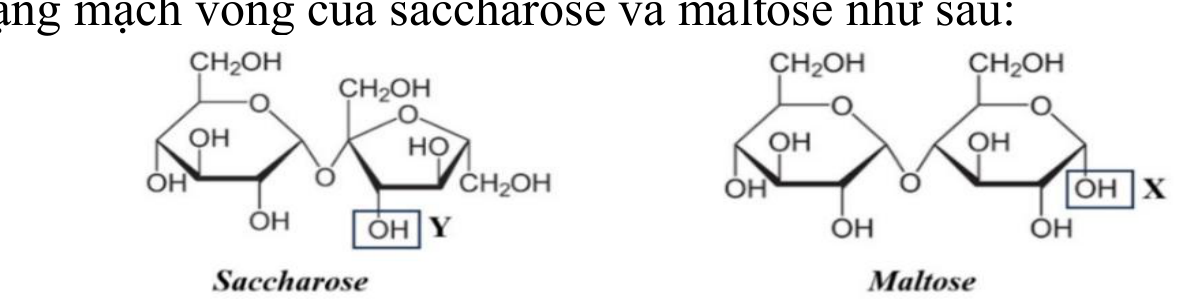
\includegraphics[width=10.5cm]{images_hungyen_12_ma0301/cau1_saccharose_maltose.png}
\end{center}
Nhận định nào sau đây đúng?
\choice
{Saccharose và maltose đều có 7 nhóm OH}
{Maltose và saccharose đều có dạng mở vòng}
{\True Nhóm OH (X) trong công thức maltose là nhóm OH hemiacetal}
{Nhóm OH (Y) trong công thức saccharose là nhóm OH hemiketal}

\loigiai{
- Trong công thức maltose, nhóm $\ce{-OH}$ ở vị trí carbon C1 anomeric của gốc glucose bên phải chưa tham gia liên kết glycosidic, đây chính là nhóm $\ce{-OH}$ hemiacetal (ký hiệu X). Nhóm này giúp gốc glucose mở vòng để tạo nhóm aldehyde $\ce{-CHO}$, có phản ứng tráng bạc.\\
- A sai vì saccharose và maltose ($\ce{C12H22O11}$) đều có 8 nhóm $\ce{-OH}$.\\
- B sai vì saccharose không có dạng mở vòng do 2 nhóm $\ce{-OH}$ anomeric đã tham gia liên kết $\alpha$-1,2-glycosidic.\\
- D sai vì nhóm $\ce{-OH}$ hemiketal ở C2 của fructose đã tạo liên kết glycosidic, nhóm $\ce{-OH}$ (Y) chỉ là nhóm alcohol thông thường.\\
\textbf{Chọn C.}
}
\end{ex}
\begin{ex}
Thuỷ phân hoàn toàn saccharose thu được X và Y. Để phân biệt X và Y, người ta sử dụng
\choice
{\True nước bromine}
{thuốc thử Tollens}
{$\ce{Cu(OH)2/OH-}$ đun nóng}
{$\ce{Cu(OH)2}$ ở nhiệt độ thường}

\loigiai{
Thuỷ phân saccharose thu được X (glucose) và Y (fructose).\\
Để phân biệt glucose và fructose, người ta sử dụng nước bromine ($\ce{Br2}$ trong nước):\\
- Glucose làm mất màu nước bromine (bị oxi hóa thành gluconic acid).\\
- Fructose không làm mất màu nước bromine do trong môi trường acid/trung tính không xảy ra sự đồng phân hóa giữa fructose và glucose.\\
\textbf{Chọn A.}
}
\end{ex}
\begin{ex}
Cho bảng nhiệt độ sôi của các chất sau ở 25$^\circ\text{C}$ và 1 bar:
\begin{center}
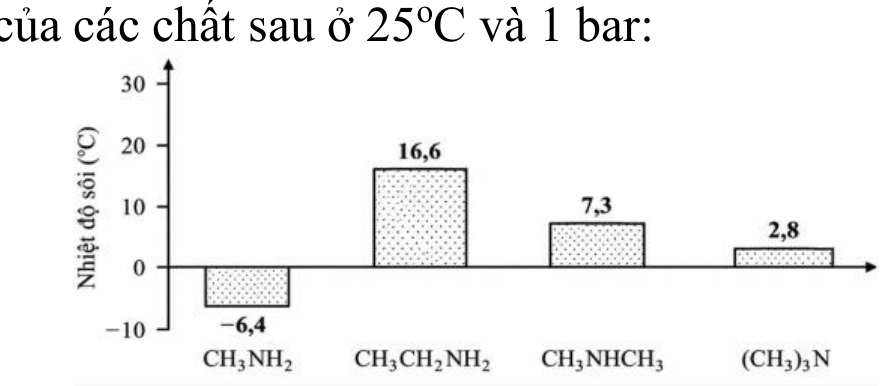
\includegraphics[width=8.5cm]{images_hungyen_12_ma0301/cau3_bieu_do_ts.png}
\end{center}
Có bao nhiêu chất ở trạng thái khí?
\choice
{3}
{1}
{2}
{\True 4}

\loigiai{
Một chất tồn tại ở trạng thái khí ở 25$^\circ\text{C}$ và 1 bar khi nhiệt độ sôi của chất đó nhỏ hơn 25$^\circ\text{C}$ ($t_{\text{sôi}} < 25^\circ\text{C}$).\\
Quan sát biểu đồ nhiệt độ sôi:\\
- $\ce{CH3NH2}$: $-6{,}4^\circ\text{C} < 25^\circ\text{C}$ (chất khí).\\
- $\ce{CH3CH2NH2}$: $16{,}6^\circ\text{C} < 25^\circ\text{C}$ (chất khí).\\
- $\ce{CH3NHCH3}$: $7{,}3^\circ\text{C} < 25^\circ\text{C}$ (chất khí).\\
- $(\ce{CH3})_3\ce{N}$: $2{,}8^\circ\text{C} < 25^\circ\text{C}$ (chất khí).\\
Cả 4 amine đều có nhiệt độ sôi thấp hơn 25$^\circ\text{C}$ nên đều ở thể khí.\\
\textbf{Chọn D.}
}
\end{ex}
\begin{ex}
Một acid béo được gọi là omega-n (khi đó n là vị trí của liên kết đôi đầu tiên tính từ nhóm methyl). Cho công thức cấu tạo của một loại acid béo X như sau:
\begin{center}

\includegraphics[width=11.5cm]{images_hungyen_12_ma0301/cau4_acid_beo.png}
\end{center}
Acid béo X thuộc loại omega nào sau đây?
\choice
{Omega-3}
{\True Omega-9}
{Omega-6}
{Omega-12}

\loigiai{
Đếm vị trí carbon từ nhóm methyl ($\ce{-CH3}$, đầu $\omega$):\\
$\ce{\overset{1}{C}H3 - \overset{2}{C}H2 - \overset{3}{C}H2 - \overset{4}{C}H2 - \overset{5}{C}H2 - \overset{6}{C}H2 - \overset{7}{C}H2 - \overset{8}{C}H2 - \overset{9}{C}H = \overset{10}{C}H - \dots - COOH}$\\
Liên kết đôi đầu tiên nằm giữa C9 và C10, tức bắt đầu ở carbon số 9 tính từ đầu methyl.\\
Do đó X thuộc loại acid béo Omega-9 (oleic acid).\\
\textbf{Chọn B.}
}
\end{ex}
\begin{ex}
Cho sơ đồ của phản ứng: $(\ce{C17H33COO})_3\ce{C3H5 + 3NaOH ->[t^\circ] 3Y}\text{ (muối)} + \ce{C3H5(OH)3}$. Công thức của muối Y là
\choice
{\True $\ce{C17H33COONa}$}
{$\ce{C17H35COONa}$}
{$\ce{C17H31COONa}$}
{$\ce{C15H31COONa}$}

\loigiai{
$(\ce{C17H33COO})_3\ce{C3H5}$ là triolein. Phản ứng xà phòng hóa trong dung dịch $\ce{NaOH}$ tạo ra muối sodium oleate $\ce{C17H33COONa}$ và glycerol.\\
\textbf{Chọn A.}
}
\end{ex}
\begin{ex}
Ở các giá trị pH khác nhau, valine có thể tồn tại chủ yếu ở các dạng khác nhau. Trong điện trường, các dạng này có khả năng dịch chuyển về các điện cực khác nhau. Cho sơ đồ biểu diễn các dạng tồn tại của valine dưới đây:
\begin{center}
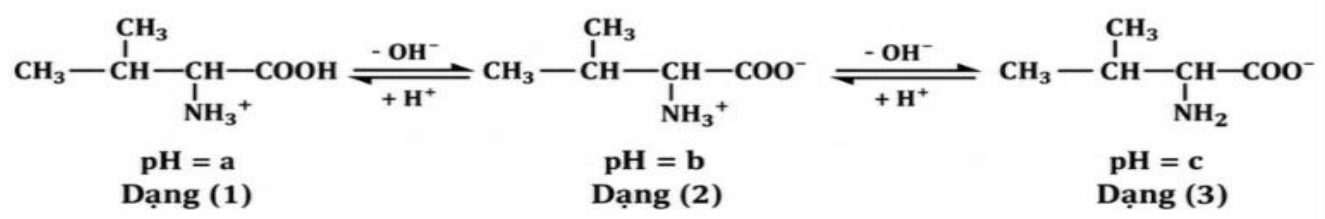
\includegraphics[width=11.5cm]{images_hungyen_12_ma0301/cau6_valine.png}
\end{center}
Phát biểu nào sau đây là sai?
\choice
{Thứ tự giá trị pH là $a < b < c$}
{\True Trong dung dịch nước, cả ba dạng (1), (2) và (3) đều có tính chất lưỡng tính}
{Ở $\text{pH} = a$, khi đặt trong điện trường, dạng (1) sẽ dịch chuyển sang cực âm}
{Dạng (1) là cation, dạng (2) là ion lưỡng cực, dạng (3) là anion}

\loigiai{
- Phát biểu B sai vì trong dung dịch nước chỉ có dạng (2) (ion lưỡng cực - zwitterion) là có tính lưỡng tính (vừa nhận proton $\ce{H+}$ ở $\ce{-COO-}$, vừa nhường proton $\ce{H+}$ ở $\ce{-NH3+}$). Dạng cation (1) chỉ có tính acid (cho $\ce{H+}$); dạng anion (3) chỉ có tính base (nhận $\ce{H+}$).\\
- Phát biểu A đúng vì cation (1) chiếm ưu thế ở môi trường acid mạnh ($\text{pH} = a$ nhỏ nhất), zwitterion (2) ở điểm đẳng điện ($\text{pH} = b \approx 6$), anion (3) ở môi trường base ($\text{pH} = c$ lớn nhất).\\
- Phát biểu C đúng vì dạng (1) mang điện tích $+1$ nên dịch chuyển về cực âm (cathode).\\
\textbf{Chọn B.}
}
\end{ex}
\begin{ex}
Ester X được tạo bởi ethyl alcohol và acetic acid có công thức cấu tạo là
\choice
{$\ce{CH3COOCH3}$}
{\True $\ce{CH3COOC2H5}$}
{$\ce{HCOOCH3}$}
{$\ce{C2H5COOC2H5}$}

\loigiai{
$\ce{CH3COOH + C2H5OH <=> CH3COOC2H5 + H2O}$.\\
Ester X là ethyl acetate: $\ce{CH3COOC2H5}$.\\
\textbf{Chọn B.}
}
\end{ex}
\begin{ex}
Cho sơ đồ: $\text{Disaccharide} \xrightarrow{+\ce{H2O},\text{ acid}, t^\circ} \text{Hỗn hợp monosaccharide} \xrightarrow{+[\ce{Ag(NH3)2}]\ce{OH}, t^\circ} \text{Bạc kim loại}$.\\
Trong quá trình trên, từ 1 mol saccharose tạo được tối đa bao nhiêu mol bạc kim loại?
\choice
{3 mol}
{2 mol}
{1 mol}
{\True 4 mol}

\loigiai{
1 mol saccharose ($\ce{C12H22O11}$) thuỷ phân tạo thành 1 mol glucose và 1 mol fructose.\\
Trong dung dịch kiềm của thuốc thử Tollens, fructose chuyển hóa thành glucose và cả 2 đều tráng bạc:\\
- $1\text{ mol glucose} \rightarrow 2\text{ mol Ag}$.\\
- $1\text{ mol fructose} \rightarrow 2\text{ mol Ag}$.\\
Tổng số mol Ag tối đa thu được $= 2 + 2 = 4\text{ mol}$.\\
\textbf{Chọn D.}
}
\end{ex}
\begin{ex}
Khi trộn dầu ăn với nước rồi để yên, người ta thấy dầu ăn tách thành một lớp nổi trên mặt nước. Nhận định nào sau đây phù hợp với hiện tượng trên?
\choice
{Dầu ăn tan trong nước và có khối lượng riêng nhỏ hơn nước}
{Dầu ăn không tan trong nước và có khối lượng riêng lớn hơn nước}
{\True Dầu ăn không tan trong nước và có khối lượng riêng nhỏ hơn nước}
{Dầu ăn tan trong nước và có khối lượng riêng lớn hơn nước}

\loigiai{
Dầu ăn (chất béo) là hợp chất không phân cực nên không tan trong nước, đồng thời có khối lượng riêng ($D \approx 0{,}8 - 0{,}9\text{ g/mL}$) nhỏ hơn nước ($D = 1{,}0\text{ g/mL}$) nên nổi lên trên.\\
\textbf{Chọn C.}
}
\end{ex}
\begin{ex}
Chất nào sau đây là thành phần chủ yếu của xà phòng?
\choice
{$\ce{CH3COOH}$}
{\True $\ce{CH3[CH2]14COONa}$}
{$\ce{CH3CH2OH}$}
{$\ce{CH3[CH2]16COOH}$}

\loigiai{
Xà phòng là hỗn hợp muối sodium hoặc potassium của acid béo.\\
$\ce{CH3[CH2]14COONa}$ (sodium palmitate - $\ce{C15H31COONa}$) là muối sodium của acid béo, là thành phần chủ yếu của xà phòng.\\
\textbf{Chọn B.}
}
\end{ex}
\begin{ex}
Dung dịch nào sau đây không có khả năng hòa tan $\ce{Cu(OH)2}$?
\choice
{\True Dung dịch ethanol}
{Nước mía}
{Nước ép quả nho chín}
{Nước ép củ cải đường}

\loigiai{
Nước mía và nước ép củ cải đường chứa saccharose; nước ép quả nho chứa glucose. Cả hai đều có nhiều nhóm $\ce{-OH}$ kề nhau nên hòa tan $\ce{Cu(OH)2}$ tạo phức xanh lam.\\
Ethanol ($\ce{C2H5OH}$) là alcohol đơn chức nên không hòa tan được $\ce{Cu(OH)2}$.\\
\textbf{Chọn A.}
}
\end{ex}
\begin{ex}
Thông thường, nếu mạch carbon của chất giặt rửa tổng hợp không phân nhánh thì chất giặt rửa đó dễ phân huỷ sinh học hơn so với mạch carbon phân nhánh. Chất giặt rửa nào sau đây dễ phân huỷ sinh học nhất?
\begin{center}
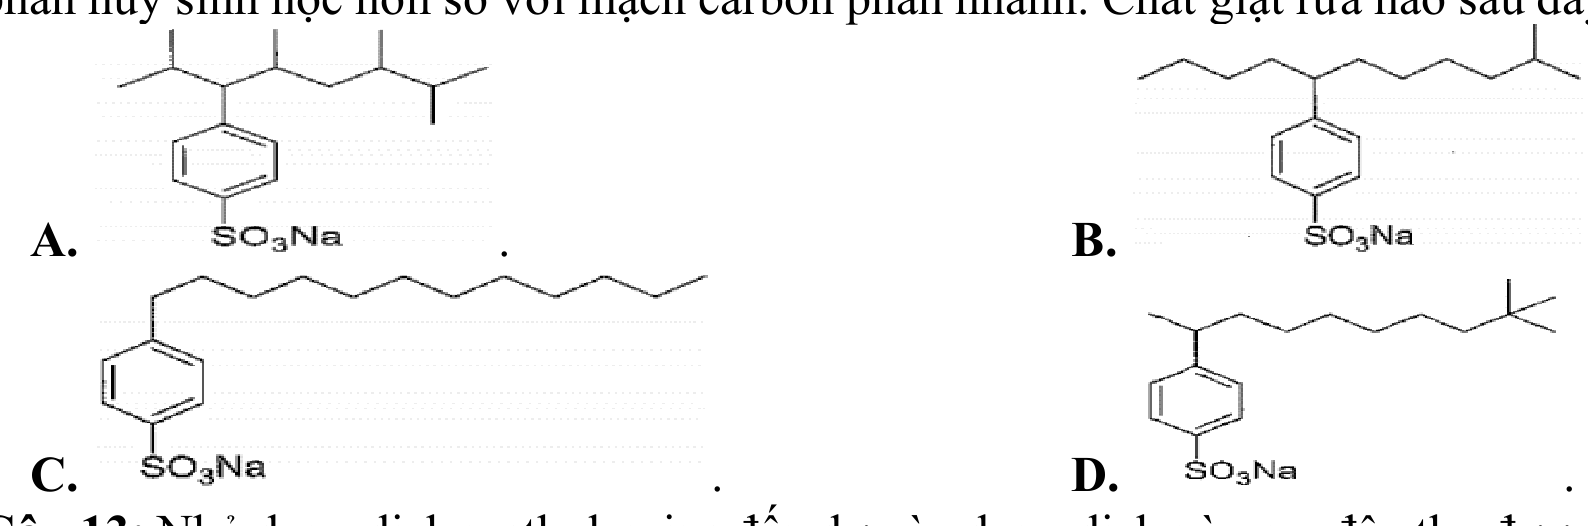
\includegraphics[width=12.5cm]{images_hungyen_12_ma0301/cau12_chat_giat_rua.png}
\end{center}
\choice
{\True Chất A}
{Chất B}
{Chất C}
{Chất D}

\loigiai{
Chất giặt rửa A có mạch alkyl kéo dài không phân nhánh (Linear Alkylbenzene Sulfonate - LAS). Chuỗi alkyl thẳng giúp vi sinh vật dễ dàng phân giải sinh học hơn rất nhiều so với chuỗi alkyl phân nhánh (B, C, D).\\
\textbf{Chọn A.}
}
\end{ex}
\begin{ex}
Nhỏ dung dịch methylamine đến dư vào dung dịch nào sau đây thu được kết tủa sau khi kết thúc phản ứng?
\choice
{\True $\ce{FeCl3}$}
{$\ce{HCl}$}
{$\ce{NaOH}$}
{$\ce{CuSO4}$}

\loigiai{
$\ce{FeCl3 + 3CH3NH2 + 3H2O -> Fe(OH)3 v} \text{ (nâu đỏ)} + \ce{3CH3NH3Cl}$.\\
Kết tủa $\ce{Fe(OH)3}$ không tan trong dung dịch methylamine dư.\\
Đối với $\ce{CuSO4}$, kết tủa $\ce{Cu(OH)2}$ ban đầu bị methylamine dư hòa tan tạo phức xanh thẫm $[\ce{Cu(CH3NH2)4}](\ce{OH})_2$.\\
\textbf{Chọn A.}
}
\end{ex}
\begin{ex}
Sắp xếp theo chiều giảm dần nhiệt độ sôi của các chất sau: methyl formate (1); acetic acid (2); ethanol (3)?
\choice
{(1) > (2) > (3)}
{(2) > (1) > (3)}
{(1) > (3) > (2)}
{\True (2) > (3) > (1)}

\loigiai{
- Acetic acid (2) có liên kết hydrogen liên phân tử bền dạng dimer $\rightarrow$ nhiệt độ sôi cao nhất ($118{,}1^\circ\text{C}$).\\
- Ethanol (3) có liên kết hydrogen liên phân tử $\rightarrow$ nhiệt độ sôi trung bình ($78{,}3^\circ\text{C}$).\\
- Methyl formate (1) là ester, không có liên kết hydrogen liên phân tử $\rightarrow$ nhiệt độ sôi thấp nhất ($31{,}5^\circ\text{C}$).\\
Thứ tự giảm dần: (2) > (3) > (1).\\
\textbf{Chọn D.}
}
\end{ex}
\begin{ex}
Trong công nghiệp sản xuất đường saccharose, người ta sử dụng phương pháp nào để tách saccharose ra khỏi dung dịch nước mía?
\choice
{Sắc kí}
{\True Kết tinh}
{Chiết}
{Chưng cất}

\loigiai{
Nước mía sau khi được lọc sạch, tẩy màu và cô đặc đến trạng thái bão hòa được làm lạnh để đường saccharose kết tinh tạo thành tinh thể đường cát trắng.\\
\textbf{Chọn B.}
}
\end{ex}
\begin{ex}
Chất nào sau đây thuộc loại polysaccharide?
\choice
{Maltose}
{Fructose}
{Glucose}
{\True Cellulose}

\loigiai{
Cellulose là polysaccharide tạo bởi nhiều gốc $\beta$-glucose.\\
\textbf{Chọn D.}
}
\end{ex}
\begin{ex}
Cho dãy các chất có công thức cấu tạo như sau:
\begin{center}
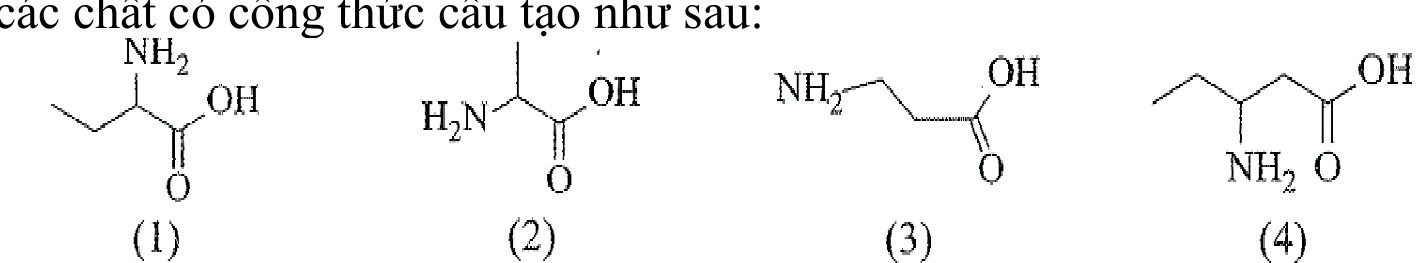
\includegraphics[width=11.5cm]{images_hungyen_12_ma0301/cau17_amino_acid.png}
\end{center}
Có bao nhiêu chất trong dãy là $\alpha$ - amino acid ?
\choice
{3}
{4}
{\True 2}
{1}

\loigiai{
$\alpha$-amino acid là amino acid có nhóm $\ce{-NH2}$ gắn ở nguyên tử carbon số 2 (carbon $\alpha$ kề nhóm $\ce{-COOH}$).\\
- Chất (1): Nhóm $\ce{-NH2}$ gắn ở carbon $\alpha$ $\rightarrow$ là $\alpha$-amino acid (2-aminobutanoic acid).\\
- Chất (2): Nhóm $\ce{-NH2}$ gắn ở carbon $\gamma$ (vị trí 4) $\rightarrow$ không phải $\alpha$.\\
- Chất (3): Nhóm $\ce{-NH2}$ gắn ở carbon $\beta$ (vị trí 3) $\rightarrow$ không phải $\alpha$.\\
- Chất (4): Nhóm $\ce{-NH2}$ gắn ở carbon $\alpha$ $\rightarrow$ là $\alpha$-amino acid (leucine).\\
Vậy có 2 chất là $\alpha$-amino acid: (1) và (4).\\
\textbf{Chọn C.}
}
\end{ex}
\begin{ex}
Phản ứng nào sau đây thuộc loại phản ứng trùng ngưng?
\begin{center}
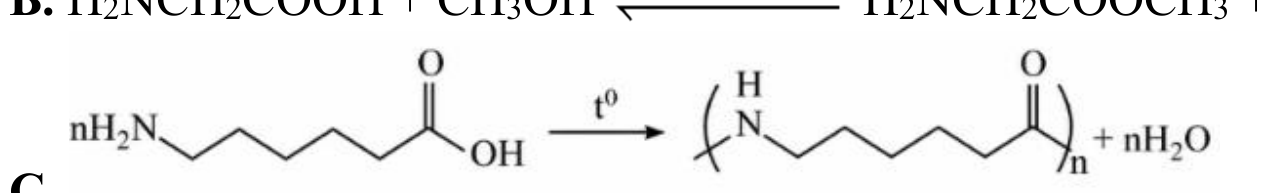
\includegraphics[width=10.0cm]{images_hungyen_12_ma0301/cau18_opt_c.png}
\end{center}
\choice
{$\ce{HCl + H2NCH(CH3)COOH -> ClH3NCH(CH3)COOH}$}
{$\ce{H2NCH2COOH + CH3OH ->[H2SO4, t^\circ] H2NCH2COOCH3 + H2O}$}
{\True Phản ứng C}
{$\ce{H2NCH(CH3)COOH + NaOH -> H2NCH(CH3)COONa + H2O}$}

\loigiai{
Phản ứng C biểu diễn quá trình trùng ngưng $\varepsilon$-aminocaproic acid (6-aminohexanoic acid) tạo thành policaproamide (nylon-6) đồng thời giải phóng nhiều phân tử nước $\ce{H2O}$.\\
\textbf{Chọn C.}
}
\end{ex}
\vspace{6pt}
\noindent
{\color{mainGreen}\textbf{\large PHẦN II. Câu trắc nghiệm đúng sai}}\\
\textit{\small Thí sinh trả lời từ câu 1 đến câu 4. Trong mỗi ý a), b), c), d) ở mỗi câu, thí sinh chọn đúng hoặc sai.}
\vspace{2pt}

\begin{ex}
Cho công thức cấu tạo của ester X như sau:
\begin{center}
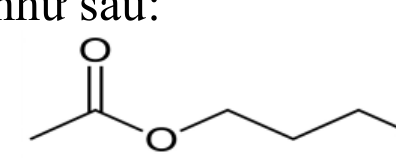
\includegraphics[width=4.5cm]{images_hungyen_12_ma0301/p2_cau1_ester.png}
\end{center}
\choiceTF
{X có tên gọi là methyl butanoate.}
{\True Phần trăm khối lượng của carbon trong ester X là 62,07\% (Kết quả làm tròn đến hàng phần trăm).}
{Phản ứng thủy phân ester X trong môi trường acid là phản ứng một chiều.}
{\True Xà phòng hoá ester X bằng dung dịch NaOH, đun nóng thu được alcohol bậc một.}

\loigiai{
Công thức cấu tạo của ester X là $\ce{CH3CH2CH2COOCH2CH3}$ (ethyl butanoate, $\ce{C6H12O2}$, $M = 116$).\\
a) \textbf{Sai.} X có tên gọi là ethyl butanoate.\\
b) \textbf{Đúng.} $\%m_{\ce{C}} = \dfrac{6 \times 12}{116} \times 100\% = 62{,}069\% \approx 62{,}07\%$.\\
c) \textbf{Sai.} Thủy phân ester trong môi trường acid là phản ứng thuận nghịch (hai chiều).\\
d) \textbf{Đúng.} Thủy phân thu được ethanol $\ce{C2H5OH}$ ($\ce{CH3CH2OH}$), là alcohol bậc một.
}
\end{ex}
\begin{ex}
Levodopa (L-dopa) là tiền chất của dopamine, thường được sử dụng như một chất thay thế dopamine để điều trị bệnh Parkinson. L-dopa có công thức cấu tạo như sau:
\begin{center}
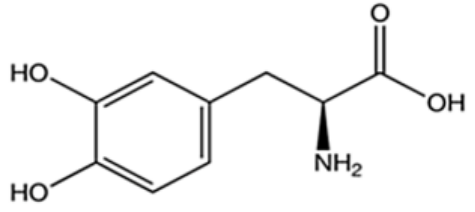
\includegraphics[width=5.0cm]{images_hungyen_12_ma0301/p2_cau2_ldopa.png}
\end{center}
\choiceTF
{\True Khi cho L-dopa phản ứng với dung dịch HCl tạo ra hợp chất hữu cơ X, trong X nguyên tố carbon chiếm 46,25\% về khối lượng (Kết quả làm tròn đến hàng phần trăm).}
{1 mol L-dopa phản ứng tối đa với 1 mol KOH.}
{\True Trong phân tử L-dopa chứa 3 loại nhóm chức.}
{\True Công thức phân tử của L-dopa là $\ce{C9H11NO4}$.}

\loigiai{
L-dopa có CTPT là $\ce{C9H11NO4}$ ($M = 197$). Cấu tạo gồm 2 nhóm $\ce{-OH}$ phenol, 1 nhóm amino $\ce{-NH2}$ và 1 nhóm carboxyl $\ce{-COOH}$.\\
a) \textbf{Đúng.} X là $\ce{C9H11NO4.HCl}$ ($\ce{C9H12ClNO4}$, $M = 233{,}5$).\\
$\%m_{\ce{C}} = \dfrac{9 \times 12}{233{,}5} \times 100\% = 46{,}2526\% \approx 46{,}25\%$.\\
b) \textbf{Sai.} 1 phân tử L-dopa có 2 nhóm $\ce{-OH}$ phenol và 1 nhóm $\ce{-COOH}$ nên 1 mol L-dopa phản ứng tối đa với 3 mol KOH.\\
c) \textbf{Đúng.} Chứa 3 loại nhóm chức: phenol, amine và carboxylic acid.\\
d) \textbf{Đúng.} CTPT là $\ce{C9H11NO4}$.
}
\end{ex}
\begin{ex}
Benzocain là chất gây tê cục bộ. Nó là thành phần hoạt chất trong nhiều loại thuốc mỡ gây tê không kê đơn như các sản phẩm trị loét miệng thương hiệu Orajel. Benzocain được tổng hợp từ nguyên liệu ban đầu là toluidin qua nhiều phản ứng, đơn giản hoá quá trình theo sơ đồ sau:
\begin{center}
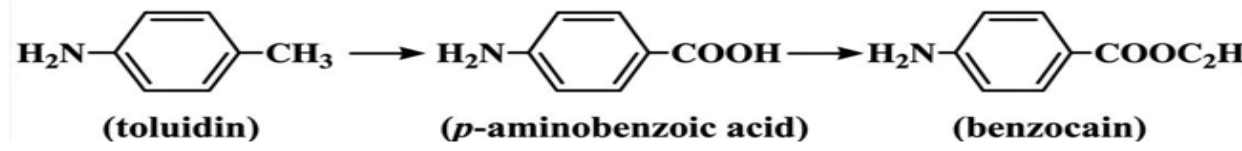
\includegraphics[width=11.5cm]{images_hungyen_12_ma0301/p2_cau3_benzocain.png}
\end{center}
\choiceTF
{Cả toluidin và benzocain đều tan tốt trong nước.}
{Benzocain có tính lưỡng tính vì vừa tác dụng với dung dịch HCl và dung dịch NaOH.}
{Trên phổ hồng ngoại của benzocain, tín hiệu (peak) ở 1700 $\text{cm}^{-1}$ đặc trưng cho liên kết C-O.}
{\True Để sản xuất một lô thuốc benzocain gồm 2000 lọ (mỗi lọ chứa 25 gam benzocain) thì cần dùng 43,2 kg toluidin. Biết hiệu suất cả quá trình là 75\%. (Kết quả cuối cùng được làm tròn đến hàng phần mười).}

\loigiai{
a) \textbf{Sai.} Cả toluidin và benzocain đều có gốc hydrocarbon thơm lớn không phân cực nên rất ít tan trong nước.\\
b) \textbf{Sai.} Benzocain có nhóm $\ce{-NH2}$ thể hiện tính base và nhóm ester bị thủy phân trong kiềm, đây không phải tính chất của chất lưỡng tính.\\
c) \textbf{Sai.} Tín hiệu ở vùng 1700 $\text{cm}^{-1}$ đặc trưng cho liên kết đôi $\ce{C=O}$ của ester (liên kết $\ce{C-O}$ hấp thụ ở 1300 -- 1000 $\text{cm}^{-1}$).\\
d) \textbf{Đúng.} $m_{\text{benzocain}} = 2000 \times 25\text{ g} = 50\text{ kg}$.\\
Sơ đồ: $\ce{C7H9N} (107) \rightarrow \ce{C9H11NO2} (165)$.\\
$m_{\text{toluidin lt}} = 50 \times \dfrac{107}{165} \approx 32{,}4242\text{ kg} \implies m_{\text{tt}} = \dfrac{32{,}4242}{0{,}75} \approx 43{,}232\text{ kg} \approx 43{,}2\text{ kg}$.
}
\end{ex}
\begin{ex}
Việc pha ethanol vào xăng góp phần hạn chế sự phụ thuộc vào nhiên liệu hóa thạch và giảm phát thải $\ce{CO2}$. Sơ đồ sau đây tóm tắt quá trình sản xuất và tiêu thụ xăng E5 (chứa 5\% ethanol về thể tích):
\begin{center}
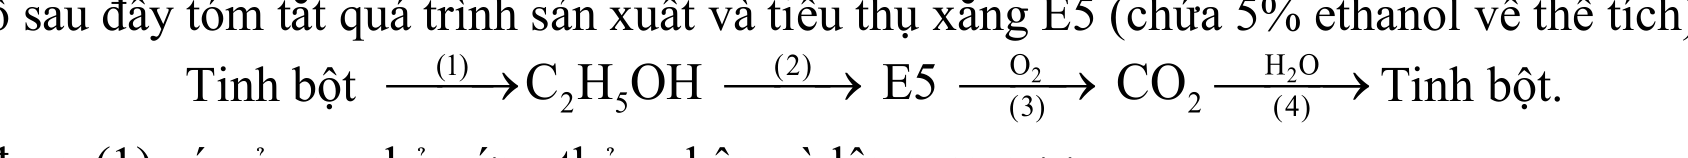
\includegraphics[width=12.5cm]{images_hungyen_12_ma0301/p2_cau4_xang_e5.png}
\end{center}
\choiceTF
{\True Giai đoạn (1) có xảy ra phản ứng thủy phân và lên men rượu.}
{\True Ở giai đoạn (2) xăng E5 được tạo ra bằng cách phối trộn 95\% thể tích xăng truyền thống (thường là xăng RON 92) với 5\% thể tích ethanol.}
{\True Phản ứng trong giai đoạn (4) xảy ra nhờ ánh sáng mặt trời và chất diệp lục trong lá cây.}
{Lên men 400 kg sắn khô (chứa 35\% khối lượng là tinh bột, phần còn lại là các chất không có khả năng lên men thành ethanol) với hiệu suất quá trình (1) là 72\%. Toàn bộ lượng ethanol sinh ra pha chế được tối đa 1435 lít xăng E5. Biết khối lượng riêng của ethanol nguyên chất là 0,8 g/mL. (Kết quả cuối cùng làm tròn đến hàng đơn vị).}

\loigiai{
a) \textbf{Đúng.} Tinh bột thủy phân thành glucose rồi lên men thành ethanol.\\
b) \textbf{Đúng.} Xăng E5 chứa 5\% thể tích ethanol sinh học và 95\% thể tích xăng khoáng.\\
c) \textbf{Đúng.} Giai đoạn (4) là phản ứng quang hợp tạo tinh bột nhờ ánh sáng mặt trời và chất diệp lục.\\
d) \textbf{Sai.} $m_{\text{tinh bột}} = 400 \times 35\% = 140\text{ kg} = 140\,000\text{ gam}$.\\
Sơ đồ: $(\ce{C6H10O5})_n (162n) \rightarrow 2n\ce{C2H5OH} (92n)$.\\
$m_{\text{ethanol tt}} = 140 \times \dfrac{92}{162} \times 72\% = 57{,}2444\text{ kg} = 57\,244{,}4\text{ g}$.\\
$V_{\text{ethanol}} = \dfrac{57\,244{,}4}{0{,}8} = 71\,555{,}5\text{ mL} = 71{,}5555\text{ L}$.\\
$V_{\text{xăng E5}} = \dfrac{71{,}5555}{0{,}05} \approx 1431\text{ lít}$ (khác 1435 lít).
}
\end{ex}
\vspace{6pt}
\noindent
{\color{mainGreen}\textbf{\large PHẦN III. Câu trắc nghiệm trả lời ngắn}}\\
\textit{\small Thí sinh trả lời từ câu 1 đến câu 6.}
\vspace{2pt}

\begin{ex}
Terephthalic acid có thể được tổng hợp từ arene X có công thức phân tử $\ce{C8H10}$, bằng cách oxi hóa X theo sơ đồ gồm hai giai đoạn:\\
(a) $x\ce{C8H10} + y\ce{KMnO4}\text{ (đun nóng)} \rightarrow z\ce{C6H4(COOK)2} + t\ce{MnO2} + g\ce{KOH} + i\ce{H2O}$\\
(b) $\ce{C6H4(COOK)2 + 2HCl -> C6H4(COOH)2 + 2KCl}$\\
Trong một thí nghiệm, từ 2,0 mL X ($D = 0{,}861\text{ g/mL}$) thu được 1,6 gam terephthalic acid. Biết $\ce{KMnO4}$ và $\ce{HCl}$ được lấy dư. Hiệu suất của quá trình tổng hợp terephthalic acid từ X là $h$\%.\\
Cho các phát biểu sau:\\
(1) Giá trị của $h$ là 59,3 (Kết quả cuối cùng làm tròn đến hàng phần mười).\\
(2) Tỉ lệ $x : g$ là 1:6.\\
(3) X có tên gọi là 1,4 - dimethylbenzene.\\
(4) Anion $^-\ce{OOCC6H4COO-}$ là một base theo thuyết Brønsted – Lowry.\\
Hãy liệt kê các phát biểu đúng theo thứ tự tăng dần. (Ví dụ: 12, 124...).

\loigiai{
- X là 1,4-dimethylbenzene ($p$-xylene) $\rightarrow$ (3) Đúng.\\
- Cân bằng phản ứng oxi hóa: $\ce{C8H10 + 4KMnO4 -> C6H4(COOK)2 + 4MnO2 + 2KOH + 2H2O}$.\\
  Tỉ lệ $x : g = 1 : 2$ $\rightarrow$ (2) Sai.\\
- Hiệu suất $h$\%: $m_{\text{X}} = 2{,}0 \times 0{,}861 = 1{,}722\text{ g} \implies n_{\text{X}} = \dfrac{1{,}722}{106}\text{ mol}$.\\
  $m_{\text{lt}} = \dfrac{1{,}722}{106} \times 166 \approx 2{,}69675\text{ g} \implies h = \dfrac{1{,}6}{2{,}69675} \times 100\% = 59{,}33\% \approx 59{,}3$ $\rightarrow$ (1) Đúng.\\
- Anion $^-\ce{OOCC6H4COO-}$ nhận $\ce{H+}$ nên là base theo Brønsted – Lowry $\rightarrow$ (4) Đúng.\\
Các phát biểu đúng: (1), (3), (4) $\rightarrow$ \textbf{Đáp án: 134}
}
\end{ex}
\begin{ex}
Chỉ số xà phòng hóa là số mg potassium hydroxide cần dùng để xà phòng hóa hoàn toàn các triglyceride và trung hòa các acid béo tự do trong 1 gam chất béo. Trong thực nghiệm, một kỹ thuật viên thực hiện thí nghiệm xác định chỉ số xà phòng hóa của một mẫu mỡ cừu theo quy trình sau:\\
Bước 1: Cân chính xác 0,50 gam mẫu mỡ cừu cho vào bình nón khô.\\
Bước 2: Thêm vào 25,00 mL dung dịch KOH $x$ M trong cồn tuyệt đối, đậy kín và đun hồi lưu trong 30 phút để đảm bảo phản ứng xảy ra hoàn toàn.\\
Bước 3: Sau khi làm nguội, thêm vài giọt phenolphthalein và chuẩn độ lượng KOH dư bằng dung dịch HCl 0,50 M. Lượng HCl cần dùng vừa đủ là 19,20 mL.\\
Bước 4: Tiến hành mẫu trắng song song (không có mỡ), cũng với 25,00 mL dung dịch KOH $x$ M trên, cần 22,70 mL dung dịch HCl 0,50 M để chuẩn độ vừa đủ KOH.\\
Chỉ số xà phòng hóa của mẫu mỡ cừu trên là bao nhiêu?

\loigiai{
- $n_{\ce{KOH}\text{ ban đầu}} = n_{\ce{HCl}\text{ mẫu trắng}} = 0{,}02270 \times 0{,}50 = 0{,}01135\text{ mol}$.\\
- $n_{\ce{KOH}\text{ dư}} = n_{\ce{HCl}\text{ mẫu thật}} = 0{,}01920 \times 0{,}50 = 0{,}00960\text{ mol}$.\\
- Lượng KOH đã phản ứng với 0,50 gam mỡ: $n_{\ce{KOH}\text{ pư}} = 0{,}01135 - 0{,}00960 = 0{,}00175\text{ mol}$.\\
- Khối lượng KOH tương ứng: $m_{\ce{KOH}} = 0{,}00175 \times 56 = 0{,}098\text{ g} = 98\text{ mg}$.\\
- Chỉ số xà phòng hóa $= \dfrac{98\text{ mg}}{0{,}50\text{ g}} = \mathbf{196}$.\\
\textbf{Đáp án: 196}
}
\end{ex}
\begin{ex}
Cho phương trình hóa học của các phản ứng được gán số thứ tự dưới đây:\\
(1) $(\ce{C15H31COO})_3\ce{C3H5 + 3NaOH ->[t^\circ] 3C15H31COONa + C3H5(OH)3}$\\
(2) $\ce{CH3COOH + C2H5OH} \xrightleftharpoons[\text{H}_2\text{SO}_4\text{ đặc},\, t^\circ]{} \ce{CH3COOC2H5 + H2O}$\\
(3) $(\ce{C17H33COO})_3\ce{C3H5 + 3H2 ->[xt, t^\circ, p] (C17H35COO)3C3H5}$\\
(4) $\ce{C6H12O6 ->[enzyme] 2CH3CH(OH)COOH}$\\
Gán số thứ tự phương trình hóa học của các phản ứng theo thứ tự tên gọi: ester hóa, hydrogen hóa, xà phòng hóa, lên men và sắp xếp theo trình tự thành dãy bốn số (ví dụ: 1234, 2341, 3421, \dots)

\loigiai{
- Ester hóa: (2)\\
- Hydrogen hóa: (3)\\
- Xà phòng hóa: (1)\\
- Lên men: (4)\\
Thứ tự: 2314.\\
\textbf{Đáp án: 2314}
}
\end{ex}
\begin{ex}
Kết quả phân tích nguyên tố của hợp chất amine đơn chức X có phần trăm khối lượng các nguyên tố như sau: $\%C = 65{,}75\%$; $\%H = 15{,}07\%$; $\%N = 19{,}18\%$. Từ chất X thực hiện sơ đồ chuyển hóa sau:\\
$\ce{X ->[+HNO2] Y ->[+CuO, t^\circ] Z ->[+I2/NaOH] T}\text{ (kết tủa màu vàng)}$\\
Cho các phát biểu sau đây:\\
(a) Ở điều kiện thường, chất X là chất khí có mùi xốc và tan tốt trong nước.\\
(b) Chất Y là alcohol bậc một, có tên thay thế là butan-2-ol.\\
(c) Chất X là amine bậc một, có tên thay thế là butan-1-amine.\\
(d) Khử chất Z bằng $\ce{NaBH4}$ thì thu được chất Y.\\
Xác định số phát biểu đúng trong các phát biểu trên.

\loigiai{
- $n_{\ce{C}} : n_{\ce{H}} : n_{\ce{N}} = \dfrac{65{,}75}{12} : \dfrac{15{,}07}{1} : \dfrac{19{,}18}{14} = 4 : 11 : 1 \implies$ X là $\ce{C4H11N}$.\\
- Z tác dụng $\ce{I2/NaOH}$ cho kết tủa vàng $\ce{CHI3}$ nên Z có nhóm $\ce{CH3-CO-}$ (butan-2-one $\ce{CH3COCH2CH3}$).\\
  $\implies$ Y là butan-2-ol $\ce{CH3CH(OH)CH2CH3}$ (alcohol bậc hai).\\
  $\implies$ X là butan-2-amine $\ce{CH3CH(NH2)CH2CH3}$ (amine bậc một).\\
- (a) Sai vì butan-2-amine là chất lỏng ở điều kiện thường.\\
- (b) Sai vì Y là alcohol bậc hai.\\
- (c) Sai vì X là butan-2-amine.\\
- (d) Đúng: khử butan-2-one bằng $\ce{NaBH4}$ thu được butan-2-ol (Y).\\
Số phát biểu đúng: 1.\\
\textbf{Đáp án: 1}
}
\end{ex}
\begin{ex}
Cho sơ đồ của phản ứng: $\text{Cellulose} \xrightarrow{+\ce{HNO3}/\ce{H2SO4}\text{ đặc}, t^\circ} \text{Cellulose trinitrate}$.\\
Phân tử khối của cellulose trinitrate là $a\cdot n$ (với $n$ là số mắt xích trong phân tử cellulose trinitrate). Xác định giá trị của $a$.

\loigiai{
Công thức mắt xích của cellulose trinitrate là $\ce{[C6H7O2(ONO2)3]}_n$ hay $\ce{[C6H7N3O11]}_n$.\\
Phân tử khối của 1 mắt xích:\\
$a = 12 \times 6 + 1 \times 7 + 14 \times 3 + 16 \times 11 = 72 + 7 + 42 + 176 = \mathbf{297}$.\\
\textbf{Đáp án: 297}
}
\end{ex}
\begin{ex}
Cho dãy các chất: tinh bột, cellulose, saccharose, glucose. Xác định số chất trong dãy có chứa liên kết glycoside trong phân tử.

\loigiai{
Liên kết glycoside có trong các phân tử disaccharide và polysaccharide:\\
- Tinh bột: có liên kết $\alpha$-1,4-glycosidic và $\alpha$-1,6-glycosidic.\\
- Cellulose: có liên kết $\beta$-1,4-glycosidic.\\
- Saccharose: có liên kết $\alpha$-1,2-glycosidic.\\
- Glucose là monosaccharide tự do, không chứa liên kết glycoside.\\
Vậy có 3 chất chứa liên kết glycoside.\\
\textbf{Đáp án: 3}
}
\end{ex}
\vspace{10pt}
\begin{center}
\textbf{------------------- HẾT -------------------}\\
\textit{\small (Học sinh không được sử dụng tài liệu. Cán bộ coi thi không giải thích gì thêm)}
\end{center}

\end{document}
